\section{\texttt{gWidgets}}

% ----------------------------------------------------------------------

\subsection{Descrição}

\begin{frame}

  \texttt{gWidgets} fornece um funções para construir interfaces
  gráficas interativas de forma fácil, rápida e portável.  \vspace{2em}

  \begin{itemize}
  \item Autor: John Verzani
  \item Lançamento: 29-Sep-2006
  \item Versão: 0.0-54
  \item URL:
    \url{http://cran.r-project.org/web/packages/gWidgets/index.html}
  \end{itemize}

\end{frame}

\begin{center}
  \frame{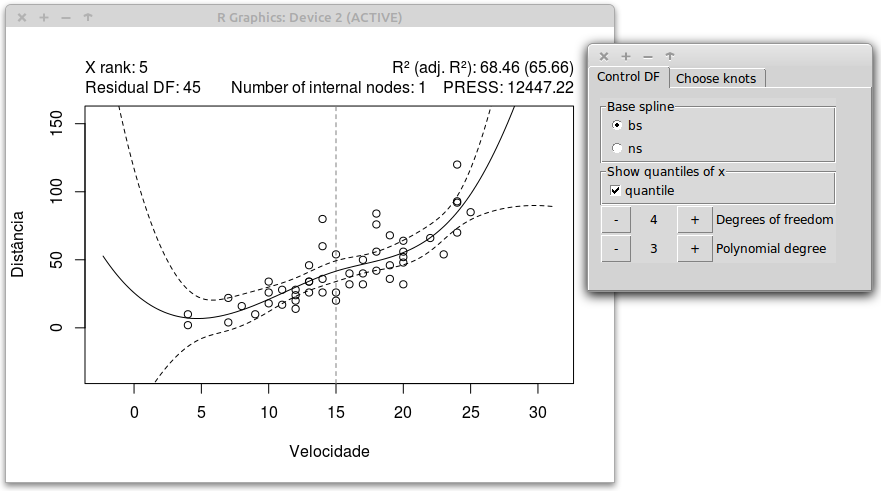
\includegraphics[width=0.95\linewidth]{./images/gui-splines.png}}
\end{center}

\begin{frame}

  Abordado nesse curso: Parte I (cap. 2-5).  \vspace{1ex}

  Verzani, J., Lawrence, M. (2012). \emph{Programming Graphical User
    Interfaces in R}, CRC Press.

  \begin{center}
    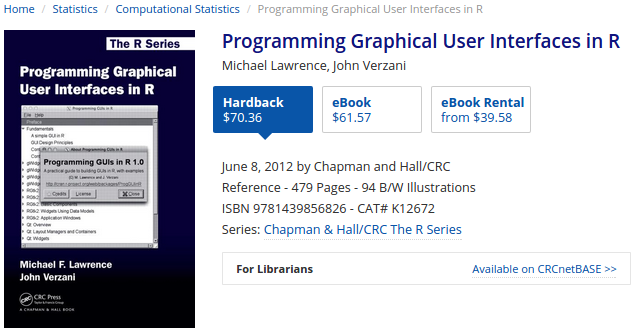
\includegraphics[width=0.8\linewidth]{./images/ProgGUI-2.png}
  \end{center}

\end{frame}

% ----------------------------------------------------------------------

\subsection{Como usar}

\frame{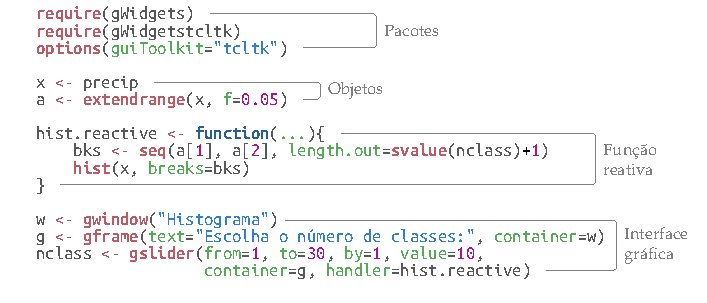
\includegraphics{./tikz/hist_slider_gWidgets-1.pdf}}
\frame{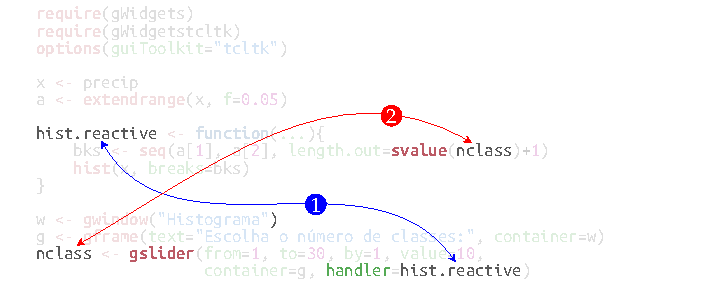
\includegraphics{./tikz/hist_slider_gWidgets-2.pdf}}

% ----------------------------------------------------------------------

\begin{frame}
  Construção de GUI centrada em 4 aspectos chave:
  \begin{enumerate}
  \item Contruir \textit{widgets} facilmente;
  \item Fazer programação de uma maneira R, com métodos S4;
  \item Facilitar a adição de \textit{handlers} para eventos na GUI;
  \item Facilitar a disposição dos elementos com \textit{containers};
  \end{enumerate}
\end{frame}

\frame{
  \begin{center}
    \resizebox{!}{0.9\textheight}{
      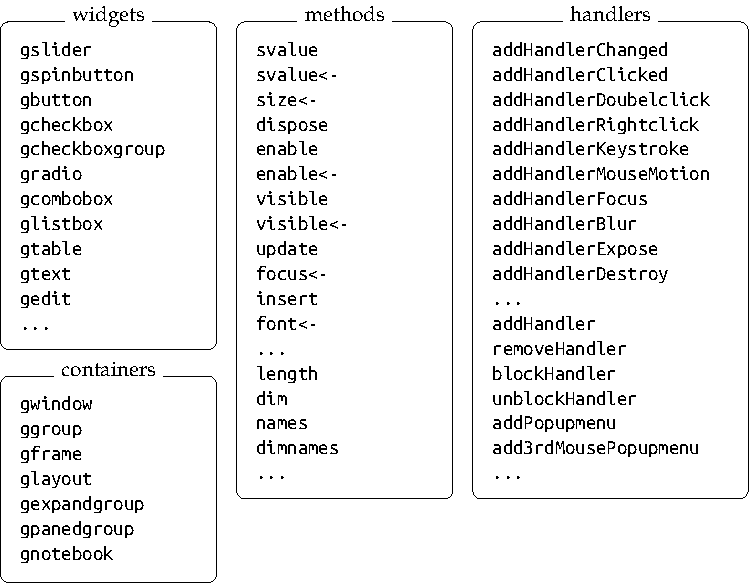
\includegraphics{./tikz/gwidgets_fun.pdf}
    }
  \end{center}
}

\begin{center}
  \frame{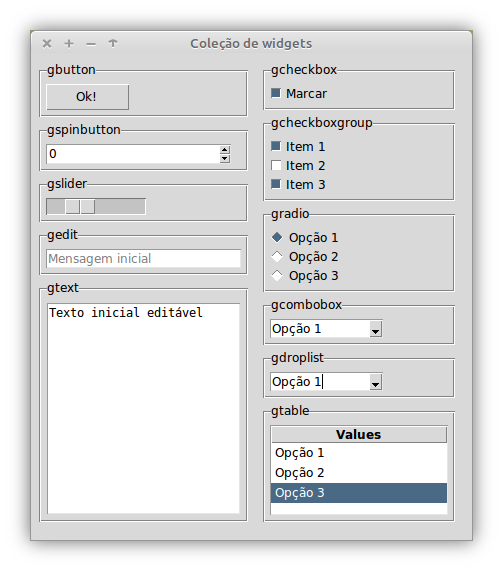
\includegraphics[width=6cm]{./images/gWidgets-widgets.png}}
\end{center}

\frame{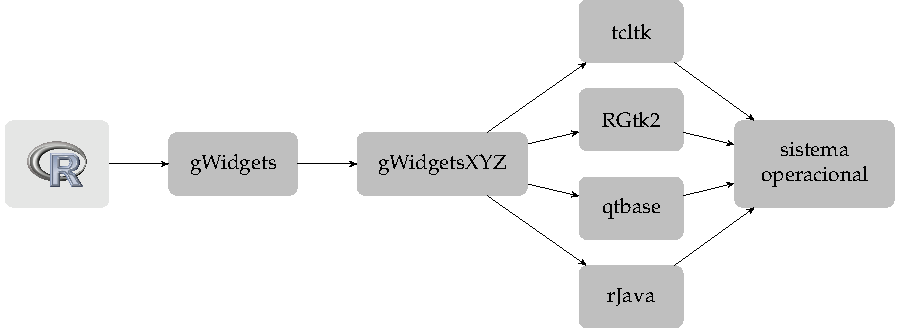
\includegraphics[width=\linewidth]{./tikz/gwidgets_working-1.pdf}}
\frame{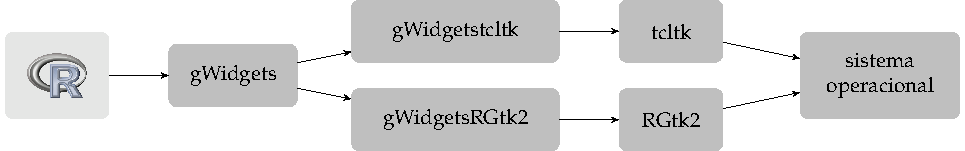
\includegraphics[width=\linewidth]{./tikz/gwidgets_working-2.pdf}}
\frame{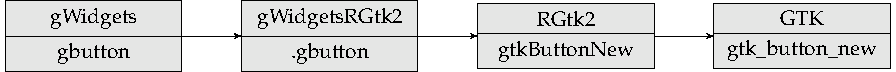
\includegraphics[width=\linewidth]{./tikz/gwidgets_working-3.pdf}}

% ----------------------------------------------------------------------

\subsection{Mais informações}

\begin{frame}
  \begin{multicols}{2}
    
    \begin{block}{Benefícios}
      \begin{itemize}
      \item Mais simples
      \item Rápido desenvolvimento
      \item Portabilide
      \end{itemize}
    \end{block}
    \vfill \columnbreak
    \begin{block}{Custos}
      \begin{itemize}
      \item Faz uma ``tradução'', perda de exatidão: mínimo denominador
        comum
      \item Portabilidade cross-toolkit tem imperfeições
      \end{itemize}
    \end{block}
  \end{multicols}

  \begin{block}{Usuários alvo}
    \begin{itemize}
    \item Não tem conhecimento detalhado de uma ferramenta de GUI
    \item Não quer aprender
    \item Mas quer fazer GUIs simples sem muito esforço
    \end{itemize}
  \end{block}

\end{frame}

% ----------------------------------------------------------------------

\subsection{Exemplos}

\begin{frame}
  Praticando:
  \begin{enumerate}
  \item \href{run:./R/gWidgets/gWidgets.R}{R Script gWidgets}
  \item \href{run:gWidgets.html}{Galeria gWidgets iguir2}
  \end{enumerate}

  \vspace{0.5cm} Algumas aplicações com o gWidgets:
  \begin{itemize}
  \item
    \href{http://cran.r-project.org/web/packages/gWidgets/vignettes/}{Galeria
      do autor}
  \item \href{https://github.com/jverzani/ProgGUIinR}{ProGUIinR Package}
  \item \href{http://www.r-bloggers.com/?s=gWidgets}{Busca no R
      Bloggers}
  \end{itemize}
\end{frame}

\begin{frame}

  Alguns pacotes que dispõem de interface gráfica:

  \begin{multicols}{2}
    \begin{block}{tcl/tk}
      \begin{itemize}
        \itemsep1pt\parskip0pt\parsep0pt
      \item
        \href{http://cran.r-project.org/web/packages/gWidgetstcltk/index.html}{\texttt{gWidgetstcltk}}
      \item
        \href{http://cran.r-project.org/web/packages/Rcmdr/index.html}{\texttt{Rcmdr}}
      \item
        \href{http://cran.r-project.org/web/packages/TeachingDemos/index.html}{\texttt{TeachingDemos}}
      \item
        \href{http://cran.r-project.org/web/packages/MetSizeR/index.html}{\texttt{MetSizeR}}
      \item
        \href{http://cran.r-project.org/web/packages/MergeGUI/index.html}{\texttt{MergeGUI}}
      \item
        \href{http://cran.r-project.org/web/packages/GrapheR/index.html}{\texttt{GrapheR}}
      \item
        \href{http://cran.r-project.org/web/packages/BiplotGUI/index.html}{\texttt{BiplotGUI}}
      \item
        \href{http://cran.r-project.org/web/packages/TestScorer/index.html}{\texttt{TestScorer}}
      \item \ldots
      \end{itemize}
    \end{block}
    \vfill \columnbreak
    \begin{block}{gtk}
      \begin{itemize}
        \itemsep1pt\parskip0pt\parsep0pt
      \item
        \href{http://cran.r-project.org/web/packages/gWidgetsRGtk2/index.html}{\texttt{gWidgetsRGtk2}}
      \item
        \href{http://cran.r-project.org/web/packages/playwith/index.html}{\texttt{playwith}}
      \item
        \href{http://cran.r-project.org/web/packages/MissingDataGUI/index.html}{\texttt{MissingDataGUI}}
      \item
        \href{http://cran.r-project.org/web/packages/GroupSeq/index.html}{\texttt{GroupSeq}}
      \item
        \href{http://cran.r-project.org/web/packages/AtelieR/index.html}{\texttt{AtelieR}}
      \item
        \href{http://cran.r-project.org/web/packages/vmsbase/index.html}{\texttt{vmsbase}}
      \item
        \href{http://cran.r-project.org/web/packages/reshapeGUI/index.html}{\texttt{reshapeGUI}}
      \item
        \href{http://cran.r-project.org/web/packages/R2STATS/index.html}{\texttt{R2STATS}}
      \item \ldots
      \end{itemize}
    \end{block}
  \end{multicols}
  
\end{frame}
